% Options for packages loaded elsewhere
\PassOptionsToPackage{unicode}{hyperref}
\PassOptionsToPackage{hyphens}{url}
%
\documentclass[
  oneside]{article}
\usepackage{amsmath,amssymb}
\usepackage{iftex}
\ifPDFTeX
  \usepackage[T1]{fontenc}
  \usepackage[utf8]{inputenc}
  \usepackage{textcomp} % provide euro and other symbols
\else % if luatex or xetex
  \usepackage{unicode-math} % this also loads fontspec
  \defaultfontfeatures{Scale=MatchLowercase}
  \defaultfontfeatures[\rmfamily]{Ligatures=TeX,Scale=1}
\fi
\usepackage{lmodern}
\ifPDFTeX\else
  % xetex/luatex font selection
\fi
% Use upquote if available, for straight quotes in verbatim environments
\IfFileExists{upquote.sty}{\usepackage{upquote}}{}
\IfFileExists{microtype.sty}{% use microtype if available
  \usepackage[]{microtype}
  \UseMicrotypeSet[protrusion]{basicmath} % disable protrusion for tt fonts
}{}
\makeatletter
\@ifundefined{KOMAClassName}{% if non-KOMA class
  \IfFileExists{parskip.sty}{%
    \usepackage{parskip}
  }{% else
    \setlength{\parindent}{0pt}
    \setlength{\parskip}{6pt plus 2pt minus 1pt}}
}{% if KOMA class
  \KOMAoptions{parskip=half}}
\makeatother
\usepackage{xcolor}
\usepackage{color}
\usepackage{fancyvrb}
\newcommand{\VerbBar}{|}
\newcommand{\VERB}{\Verb[commandchars=\\\{\}]}
\DefineVerbatimEnvironment{Highlighting}{Verbatim}{commandchars=\\\{\}}
% Add ',fontsize=\small' for more characters per line
\usepackage{framed}
\definecolor{shadecolor}{RGB}{248,248,248}
\newenvironment{Shaded}{\begin{snugshade}}{\end{snugshade}}
\newcommand{\AlertTok}[1]{\textcolor[rgb]{0.94,0.16,0.16}{#1}}
\newcommand{\AnnotationTok}[1]{\textcolor[rgb]{0.56,0.35,0.01}{\textbf{\textit{#1}}}}
\newcommand{\AttributeTok}[1]{\textcolor[rgb]{0.13,0.29,0.53}{#1}}
\newcommand{\BaseNTok}[1]{\textcolor[rgb]{0.00,0.00,0.81}{#1}}
\newcommand{\BuiltInTok}[1]{#1}
\newcommand{\CharTok}[1]{\textcolor[rgb]{0.31,0.60,0.02}{#1}}
\newcommand{\CommentTok}[1]{\textcolor[rgb]{0.56,0.35,0.01}{\textit{#1}}}
\newcommand{\CommentVarTok}[1]{\textcolor[rgb]{0.56,0.35,0.01}{\textbf{\textit{#1}}}}
\newcommand{\ConstantTok}[1]{\textcolor[rgb]{0.56,0.35,0.01}{#1}}
\newcommand{\ControlFlowTok}[1]{\textcolor[rgb]{0.13,0.29,0.53}{\textbf{#1}}}
\newcommand{\DataTypeTok}[1]{\textcolor[rgb]{0.13,0.29,0.53}{#1}}
\newcommand{\DecValTok}[1]{\textcolor[rgb]{0.00,0.00,0.81}{#1}}
\newcommand{\DocumentationTok}[1]{\textcolor[rgb]{0.56,0.35,0.01}{\textbf{\textit{#1}}}}
\newcommand{\ErrorTok}[1]{\textcolor[rgb]{0.64,0.00,0.00}{\textbf{#1}}}
\newcommand{\ExtensionTok}[1]{#1}
\newcommand{\FloatTok}[1]{\textcolor[rgb]{0.00,0.00,0.81}{#1}}
\newcommand{\FunctionTok}[1]{\textcolor[rgb]{0.13,0.29,0.53}{\textbf{#1}}}
\newcommand{\ImportTok}[1]{#1}
\newcommand{\InformationTok}[1]{\textcolor[rgb]{0.56,0.35,0.01}{\textbf{\textit{#1}}}}
\newcommand{\KeywordTok}[1]{\textcolor[rgb]{0.13,0.29,0.53}{\textbf{#1}}}
\newcommand{\NormalTok}[1]{#1}
\newcommand{\OperatorTok}[1]{\textcolor[rgb]{0.81,0.36,0.00}{\textbf{#1}}}
\newcommand{\OtherTok}[1]{\textcolor[rgb]{0.56,0.35,0.01}{#1}}
\newcommand{\PreprocessorTok}[1]{\textcolor[rgb]{0.56,0.35,0.01}{\textit{#1}}}
\newcommand{\RegionMarkerTok}[1]{#1}
\newcommand{\SpecialCharTok}[1]{\textcolor[rgb]{0.81,0.36,0.00}{\textbf{#1}}}
\newcommand{\SpecialStringTok}[1]{\textcolor[rgb]{0.31,0.60,0.02}{#1}}
\newcommand{\StringTok}[1]{\textcolor[rgb]{0.31,0.60,0.02}{#1}}
\newcommand{\VariableTok}[1]{\textcolor[rgb]{0.00,0.00,0.00}{#1}}
\newcommand{\VerbatimStringTok}[1]{\textcolor[rgb]{0.31,0.60,0.02}{#1}}
\newcommand{\WarningTok}[1]{\textcolor[rgb]{0.56,0.35,0.01}{\textbf{\textit{#1}}}}
\usepackage{longtable,booktabs,array}
\usepackage{calc} % for calculating minipage widths
% Correct order of tables after \paragraph or \subparagraph
\usepackage{etoolbox}
\makeatletter
\patchcmd\longtable{\par}{\if@noskipsec\mbox{}\fi\par}{}{}
\makeatother
% Allow footnotes in longtable head/foot
\IfFileExists{footnotehyper.sty}{\usepackage{footnotehyper}}{\usepackage{footnote}}
\makesavenoteenv{longtable}
\usepackage{graphicx}
\makeatletter
\def\maxwidth{\ifdim\Gin@nat@width>\linewidth\linewidth\else\Gin@nat@width\fi}
\def\maxheight{\ifdim\Gin@nat@height>\textheight\textheight\else\Gin@nat@height\fi}
\makeatother
% Scale images if necessary, so that they will not overflow the page
% margins by default, and it is still possible to overwrite the defaults
% using explicit options in \includegraphics[width, height, ...]{}
\setkeys{Gin}{width=\maxwidth,height=\maxheight,keepaspectratio}
% Set default figure placement to htbp
\makeatletter
\def\fps@figure{htbp}
\makeatother
\setlength{\emergencystretch}{3em} % prevent overfull lines
\providecommand{\tightlist}{%
  \setlength{\itemsep}{0pt}\setlength{\parskip}{0pt}}
\setcounter{secnumdepth}{-\maxdimen} % remove section numbering
\newlength{\cslhangindent}
\setlength{\cslhangindent}{1.5em}
\newlength{\csllabelwidth}
\setlength{\csllabelwidth}{3em}
\newlength{\cslentryspacingunit} % times entry-spacing
\setlength{\cslentryspacingunit}{\parskip}
\newenvironment{CSLReferences}[2] % #1 hanging-ident, #2 entry spacing
 {% don't indent paragraphs
  \setlength{\parindent}{0pt}
  % turn on hanging indent if param 1 is 1
  \ifodd #1
  \let\oldpar\par
  \def\par{\hangindent=\cslhangindent\oldpar}
  \fi
  % set entry spacing
  \setlength{\parskip}{#2\cslentryspacingunit}
 }%
 {}
\usepackage{calc}
\newcommand{\CSLBlock}[1]{#1\hfill\break}
\newcommand{\CSLLeftMargin}[1]{\parbox[t]{\csllabelwidth}{#1}}
\newcommand{\CSLRightInline}[1]{\parbox[t]{\linewidth - \csllabelwidth}{#1}\break}
\newcommand{\CSLIndent}[1]{\hspace{\cslhangindent}#1}
\ifLuaTeX
\usepackage[bidi=basic]{babel}
\else
\usepackage[bidi=default]{babel}
\fi
\babelprovide[main,import]{spanish}
% get rid of language-specific shorthands (see #6817):
\let\LanguageShortHands\languageshorthands
\def\languageshorthands#1{}
\usepackage{makeidx}
\makeindex
\usepackage{graphicx}
\usepackage{tikz}
\usepackage{atbegshi}
\usepackage{amsthm}
\newtheorem{definition}{Definición}[section]

\AtBeginDocument{
    \AtBeginShipoutNext{
        \AtBeginShipoutUpperLeft{
            \put(\dimexpr\paperwidth/2-\textwidth/2\relax, -650){
                \makebox[\textwidth]{
                    
\includegraphics[width=0.45\textwidth]{cure_udelar.png}  % Adjust width as needed
                    \hfill
                    
\includegraphics[width=0.405\textwidth]{logoMEDIA.jpeg} % Make it 90% smaller
                }
            }
        }
    }
}

\usepackage{amsthm}
\ifLuaTeX
  \usepackage{selnolig}  % disable illegal ligatures
\fi
\IfFileExists{bookmark.sty}{\usepackage{bookmark}}{\usepackage{hyperref}}
\IfFileExists{xurl.sty}{\usepackage{xurl}}{} % add URL line breaks if available
\urlstyle{same}
\hypersetup{
  pdftitle={Entrega: curso de datos extremales},
  pdfauthor={Laura Montaldo, CI: 3.512.962-7},
  pdflang={es},
  hidelinks,
  pdfcreator={LaTeX via pandoc}}

\title{Entrega: curso de datos extremales}
\author{Laura Montaldo, CI: 3.512.962-7}
\date{2024-04-09}

\begin{document}
\maketitle

\newtheorem{theorem}{Teorema}

\newpage

\thispagestyle{empty}

\maketitle

\newpage

\tableofcontents

\newpage

\hypertarget{resumen}{%
\section{Resumen}\label{resumen}}

Your abstract goes here.

\newpage

\section{Motivación y objetivo del estudio}

Siguiendo a Perera, Segura, y Crisci (2021), se dice que tenemos datos
extremos cuando cada dato corresponde al máximo o mínimo de varios
registros. Son un caso particular de evento raro o gran desviación
respecto a la media. Es por este motivo que en una gran variedad de
dominios disciplinares suele ser de gran interés el trabajo con datos
extremos. Además, admiten diversos enfoques. La teoría `más' clásica de
estadística de datos extremos se basa en los trabajos de Fréchet,
Gumbel, Weibull, Fisher, Tippett, Gnedenko, entre otros. En este
estudio, el foco va a estar puesto en esquemas que extienden a las
distribuciones extremales clásicas.

Los índices de \(S\&P\) son una familia de índices de renta
variable\footnote{En inglés se llaman equity indices} diseñados para
medir el rendimiento del mercado de acciones en Estados Unidos que
cotizan en bolsas estadounidenses. Ésta familia de índices está
compuesta por una amplia variedad de índices basados en tamaño, sector y
estilo. Los índices están ponderados por el criterio
\textit{float-adjusted market capitalization} (FMC). Además, se disponen
de índices ponderados de manera equitativa y con límite de
capitalización de mercado, como es el caso del \(S\&P\:500\). Este este
sentido, el \(S\&P 500\) entraría en el conjunto de índices ponderados
por capitalización bursátil ajustada a la flotación (ver
\href{http://www.overleaf.com}{\textcolor{blue}{$S\&P$ Dow Jones Indices}}).
El mismo mide el rendimiento del segmento de gran capitalización del
mercado estadounidense. Es considerado como un indicador representativo
del mercado de renta variable de los Estados Unidos, y está compuesto
por 500 empresas constituyentes.

Se busca crear un indicador de una posible crisis bursátil. Como
variable de referencia de toma la relación de precios al cierre de ayer
sobre la de hoy

\begin{equation}
Indicador_t=\frac{Precio_{t-1}}{Precio_t},\quad\text{para}\; t=1,...,T \label{eq:ind}
\end{equation} \vspace{0.5cm}

Interpretación del Indicador:

\begin{itemize}
\item Si el $Indicador_t$    $\leq$ 1, el precio de cierre de hoy es mayor o igual que el de ayer, lo cual podría ser considerado una señal positiva.
\item Si el $Indicador_t$ > 1, el precio de cierre de hoy es menor que el de ayer, lo cual podría considerarse una señal de alerta.
\end{itemize}

\newpage

En las siguiente figuras se muestra la evolución histórica desde la
fecha 03/01/1928 hasta 08/12/2023 del precio al cierre del día del
indicar S\&P 500.

\newpage

\section{Marco teorico}

\subsection{Teoría clásica}
\subsubsection{La teoría asintótica clásica, las distribuciones extremales y sus dominios de atracción}

Se parte de suponer que \(X\) e \(Y\) son variables aleatorias
\(i.i.d\), cuyas distribuciones son \(F\) y \(G\), respectivamente.
Entonces la variable

\begin{equation}
max(X,Y)
\end{equation}

tiene por distribución la función \(H\) definida por

\begin{equation}
H(t)= F(t) G(t)
\end{equation}

Entonces, si se tiene datos \(X_1,...,X_n\) \(i.i.d\) con distribución
\(F\), entonces

\begin{equation}
X_n^* = max (X_1,...,X_n)
\end{equation}

tiene distribución \(F_n^*\) dada por

\begin{equation}
F_n^* (t)= F(t)^n
\end{equation}

Dado que no en todo los casos es viable o manejable conocer la
distribución \(F\) y por lo tanto, también la de distribución \(F_n^*\),
en una línea de trabajo similar a la que aporta el Teorema Central del
Límite en la estadística de valores medios, se emplea un teorema para
aproximar \(F_n^{*}\) por distribuciones más sencillas. Este es el
Teorema de Fischer-Tippet-Gnedenko (FTG).

\hypertarget{observaciuxf3n-1}{%
\subparagraph{Observación 1}\label{observaciuxf3n-1}}

Como \(X_1,...,X_n\) se supone \(i.i.d\), si definimos \(Y_i = -X_i\)
para todo valor de \(i\), entonces \(Y_1,...,Y_n\) es \(i.i.d\) y además

\begin{equation}
min(X_1,...,X_n) = - max(Y_1,...,Y_n)
\end{equation}

la teoría asintótica de los mínimos de datos \(i.i.d\) se reduce a la de
los máximos, razón por la que nos concentramos aquí en estudiar el
comportamiento asintótico de los máximos exclusivamente.

\hypertarget{definiciuxf3n-1-las-distribuciones-extremales}{%
\paragraph{Definición 1: Las distribuciones
extremales}\label{definiciuxf3n-1-las-distribuciones-extremales}}

Las distribuciones extremales son tres: la distribución de Gumbel; la
distribución de Weibull; la distribución de Fréchet. En su versión
standard o típica se definen del modo siguiente.

\hypertarget{distribuciuxf3n-de-gumbel}{%
\subparagraph{Distribución de Gumbel}\label{distribuciuxf3n-de-gumbel}}

Se dice que una variable tiene distribución de Gumbel si su distribución
es:

\begin{equation}
\Lambda(x) = exp\{-e^{-x}\} \quad\text{para todo}\; x \;\text{real} 
\end{equation}

\hypertarget{distribuciuxf3n-de-weibull}{%
\paragraph{Distribución de Weibull}\label{distribuciuxf3n-de-weibull}}

Se dice que una variable tiene distribución de Weibull de orden
\(\alpha>0\) si su distribución es:

\begin{equation}
\Psi_{\alpha}(x)=\begin{cases}
exp{-(-x)^{\alpha}} & si\;x<0\\
1 & \text{en otro caso}
\end{cases}
\end{equation}

\hypertarget{distribuciuxf3n-de-fruxe9chet}{%
\paragraph{Distribución de
Fréchet}\label{distribuciuxf3n-de-fruxe9chet}}

Se dice que una variable tiene distribución de Fréchet de orden
\(\alpha>0\) si su distribución es:

\begin{equation}
\Phi_{\alpha}(x)=\begin{cases}
exp\{-x^{-\alpha}\} & si\;x>0\\
0 & \text{en otro caso}
\end{cases}
\end{equation}

\textbf{Nota:}

Como los máximos en general son valores grandes, importa particularmente
observar el comportamiento de estas distribuciones para \(x\) tendiendo
a infinito. El límite es 1 como en toda distribución. Pero VA MAS RAPIDO
a 1 la Weibull, luego la Gumbel y luego la Fréchet. Esto es indicio que
la Fréchet modela datos ``más extremos'', máximos de datos de colas más
pesadas que la Gumbel y esta que la Weibull. Más adelante veremos esto
más precisamente. En la Fréchet, la velocidad de convergencia a 1 crece
al aumentar el orden. En cambio en la Weibull el orden afecta la
velocidad con que va a 0 cuando \(x\) tiende a menos infinito, que crece
cuanto mayor el orden. Esto quedará más claro con el Teorema 1 del
curso. La visualización de las densidades de cada tipo quizás ayude a
comprender mejor los pesos relativos de las colas.

\newpage

A estas versiones standard se las puede extender agregando un parámetro
de recentramiento (\(\mu\)) y un parámetro de escala (\(\beta\)).

\begin{itemize}
\item Se dice que $X$ tiene distribución $\Lambda^{(c,\beta)}$ si
$$
X=\mu+\beta Y,
$$
donde $Y$ tiene distribución $\Lambda$.
\item Se dice que $X$ tiene distribución $\Psi_{\alpha}^{(\mu,\beta)}$ si 
$$
X=\mu+\beta Y,
$$
donde $Y$ tiene distribución $\Psi_{\alpha}$.

\item  Se dice que $X$ tiene distribución $\Phi_{\alpha}^{(\mu,\beta)}$ 
$$
X=\mu+\beta Y
$$
donde $Y$ tiene distribución $\Phi_{\alpha}$
\end{itemize}

En general, es en este sentido que diremos que una variable es Gumbel,
Weibull o Fréchet (incluyendo recentramiento y reescalamiento), pero en
cálculos donde los parámetros \(\mu\) y \(\beta\) no sean relevantes,
por simplicidad, usaremos las versiones standard.

\newpage

El siguiente teorema vincula las distribuciones extremales en sus
formatos standard y resulta de gran utilidad práctica sobre todo al
hacer tests de ajustes, etc.

\hypertarget{teorema-1-relaciones-entre-las-versiones-standard-de-las-distribuciones-extremales}{%
\subparagraph{Teorema 1: Relaciones entre las versiones standard de las
distribuciones
extremales}\label{teorema-1-relaciones-entre-las-versiones-standard-de-las-distribuciones-extremales}}

\(X\) tiene distribución \(\Phi_{\alpha}(x)\) si y sólo si \((-1/X)\)
tiene distribución \(\Psi_{\alpha}(x)\) si y sólo si \(log(X^{\alpha})\)
tiene distribución \(\Lambda\).

\textbf{Nota:}

En otros contextos de la Estadística (en particular en alguna rutinas
del \textbf{R}), se le llama Weibull a una variable que corresponde a
\(-X\), con X Weibull como definimos nosotros.

\textbf{Observación 5:}

Recordamos que la función Gamma (\(\Gamma\)), que extiende la función
factorial (\(\Gamma(n)=n-1!\) para todo \(n\) natural) definida por

\begin{equation}
\Gamma(u)=\int_0^{\infty}t^{u-1}e^{-t}dt
\end{equation}

es una función disponible tanto en el software \textbf{R} como en
planillas de cálculo, etc.

\hypertarget{teorema-2-tres-en-uno-algunos-datos-de-las-distribuciones-extremales.}{%
\subparagraph{Teorema 2: (Tres en uno) Algunos datos de las
distribuciones
extremales.}\label{teorema-2-tres-en-uno-algunos-datos-de-las-distribuciones-extremales.}}

\hypertarget{parte-1}{%
\subparagraph{Parte 1}\label{parte-1}}

Si \(X\) tiene distribución \(\Lambda^{(\mu,\beta)}\) entonces tiene:

\begin{itemize}
  \item[a)] Valor esperado: $E(X) = \mu + \beta\gamma$, donde $\gamma$ es la constante de Euler-Mascheroni, cuyo valor aproximado es $0.5772156649$.
  \item[b)] Moda: $\mu$
  \item[c)] Mediana: $\mu - \beta \log(\log 2) \approx \mu - 0.36651 \beta$.
  \item[d)] Desviación estándar: $\beta \pi \sqrt{6} \approx 1.2825 \beta$.
  \item[e)] Si $X^+ = \max(X,0)$, entonces $E(X^{+k})$ es finito para todo valor de $k$ natural.
  \item[f)] Para simular computacionalmente $X$, se puede tomar $U$ uniforme en $(0,1)$ y hacer $$X = \mu - \beta \log(-\log U)$$.
\end{itemize}

\hypertarget{parte-2}{%
\paragraph{Parte 2}\label{parte-2}}

Si \(X\) tiene distribución \(\Psi_{\alpha}^{(\mu,\beta)}\) entonces
tiene:

\begin{itemize}
  \item[a)] Valor esperado: $E(X) = \mu + \beta\Gamma(1+1/\alpha)$.
  \item[b)] Moda: $\mu$ si $\alpha\leq 1$ y $\mu-\beta\{(\alpha-1)/\alpha\}^{(1/\alpha)}$ si $\alpha>1$.
  \item[c)] Mediana: $\mu - \beta \log(2)^{(1/\alpha)}$.
  \item[d)] Desviación estándar: $\beta\{\Gamma(1+2/\alpha)-\Gamma(1+1/\alpha)^2\}^{1/2}$.
\end{itemize}

\hypertarget{parte-3}{%
\paragraph{Parte 3}\label{parte-3}}

Si \(X\) tiene una distribución \(\Phi_{\alpha}^{(\mu, \beta)}\)
entonces se tiene:

\begin{itemize}
  \item[a)] Valor esperado: $E(X) = \mu + \beta\Gamma(1-1/\alpha)$ si $\alpha > 1$, $\infty$ en caso contrario.
  \item[b)] Moda: $\mu + \beta\Gamma(1-1/\alpha)$ si $\alpha>1$.
  \item[c)] Mediana: $\mu + \beta \log(2)^{(-1/\alpha)}$.
  \item[d)] Desviación estándar: $\beta|\Gamma(1-2/\alpha)-\Gamma(1-1/\alpha)^2|$ si $\alpha>2$, $\infty$ si $1<\alpha \leq 2$.
\end{itemize}

\textbf{Observación 6.}

El item e de la Parte 1 es trivialmente cierto para Weibull y, tomando
en cuenta el item a) de la Parte 3, es claramente falso para Fréchet.

\textbf{Observación 7.}

El item f de la Parte 1 en conjunto con el Teorema 1 provee de fórmulas
sencillas para simular computacionalmente distribuciones Weibull o
Fréchet.

\textbf{Observación 8.}

En una simple planilla de cálculo se generaron mil números aleatorios y
aplicando el item f de la Parte 1 se simularon mil variables Gumbel
standard \(i.i.d\), calculándose su promedio, su desviación standard
empírica y su mediana empírica. Se obtuvo:

\begin{table}[h]
\centering
\begin{tabular}{|c|c|}
\hline
Promedio & -0.558355214 \\ \hline
Desvio Standard & 1.238412395 \\ \hline
Mediana & -0.3755425075 \\ \hline
\end{tabular}
\end{table}

Observar que están cerca del valor esperado, desvío standard y mediana
de la Gumbel standard.

\newpage

A continuación presentaremos el Teorema medular de esta primera parte,
expresado de la manera más llana posible. Veremos posteriormente algunos
detalles con más cuidado. En particular, veremos que la continuidad de
la distribución \(F\) no es una hipótesis real (ni es necesaria ni es
suficiente, por eso la entrecomillamos), pero ayuda a visualizar que no
vale el teorema para toda distribución \(F\), así como veremos con
cierto detalle más adelante\ldots{}

\hypertarget{teorema-3-fischer-tippet-gnedenko-ftg}{%
\subparagraph{Teorema 3: Fischer-Tippet-Gnedenko
(FTG)}\label{teorema-3-fischer-tippet-gnedenko-ftg}}

Si \(X_1,...,X_n\quad .i.i.d\) con distribución \(F\) ``continua'',
llamamos \(F_n^*\) a la distribución de \(max(X_1,...,X_n)\) y \(n\) es
grande, entonces existen \(\mu\) real y \(\beta>0\) tales que alguna de
las siguientes tres afirmaciones es correcta:

\begin{itemize}
  \item[1)] $F_n^*$ se puede apromixar por la distribución de $\mu+\beta Y$ con $Y$ variable con distribución $\Lambda$.
  \item[2)] Existe $\alpha>0$ tal que $F_n^*$ se puede aproximar por la distribución de $\mu+\beta Y$ con $Y$ variable con distribución $\Phi_{\alpha}$. 
  \item[3)] Existe $\alpha>0$ tal que $F_n^*$ se puede aproximar por la distribución de $\mu+\beta Y$ con $Y$ variable con distribución $\Phi_{\alpha}$.
\end{itemize}

Lo anterior equivale a decir que la distribución del máximo de datos
\textit{continuos} e \(iid\), si \(n\) es grande, puede aproximarse por
una Gumbel, una Fréchet o una Weibull.

\textbf{Observación 9.}

Como veremos con cierto detalle, cuál de las tres aproximaciones es la
válida depende de cómo sea la distribución \(F\). En este sentido,

\begin{itemize}
\item cuando $F$ sea normal entonces $F_n^*$ se puede aproximar como una Gumbel
\item cuando $F$ sea uniforme, se puede aproximar $F_n^*$ como una Weibull
\item cuando $F$ sea Cauchy entonces $F_n^*$ se puede aproximar por una Fréchet
\end{itemize}

Más precisamente, cuál de las tres aproximaciones es la aplicable
depende de la cola de \(F\) (los valores de \(F(t)\) para valores
grandes de \(t\)).

En concreto, Weibull aparece cuando \(F\) es la distribución de una
variable acotada por arriba (como la Uniforme), Gumbel para
distribuciones de variables no acotadas por arriba pero con colas muy
livianas (caso Exponencial y Normal) y Fréchet para colas pesadas (caso
Cauchy)\footnote{Si bien  la hipótesis de continuidad de $F$ no es esencial, si $F$ tiene
la distribución Binomial o Poisson, por ejemplo, no se puede aplicar ninguna de las tres aproximaciones anteriores.}.

\textbf{Observación 10.}

Como consecuencia del FTG si se tienen datos de máximos, las
distribuciones extremales son ``candidatas'' razonables para proponer en
un ajuste. Sin embargo no debe pensarse que siempre se va a lograr
ajustar a una de las tres distribuciones extremales, ya que hay al menos
dos causas evidentes que podrían desbaratar la aplicación del FTG:

\begin{itemize}
\item Que la cantidad de registros es lo suficientemente grande
\item Que los registros que se consideran al calcular cada máximo no sean $i.i.d$. Al final del capítulo 2 se verá que esto puede subsanarse con versiones más generales del FTG.
\end{itemize}

Por consiguiente el FTG alienta a intentar ajustar datos extremales a
una de las tres distribuciones extremales, pero no siempre un tal ajuste
dará un resultado afirmativo.

\textbf{Ejemplo 1.}

Veamos un ejemplo de ajuste. Los siguientes datos corresponden a los
valores, en 80 puntos geográficos distintos de la región parisina, del
máximo estival del contaminante atmosférico \(O_3\) (no perceptible
sensorialmente y con impacto sanitario serio). Cada datos es el máximo
registro en cada sensor a lo largo de todo un verano; el contaminante se
mide diariamente, por lo cual cada uno de nuestros 80 datos es el máximo
de unas 100 lecturas diarias).

Los valores se miden en unidades de referencia standarizadas que, en
particular, permiten comparar las medidas de lugares diferentes,
independientemente de variables relevantes como altura e incidencia
solar, por trabajo previo de calibración. El objetivo del estudio en
esta etapa es conocer la distribución de éstos datos y en particular
estimar la probabilidad de que el máximo estival en los 80 puntos supere
el valor 50 (correspondiente a existencia de riesgo moderado). Veamos
los datos que tenemos:

\begin{Shaded}
\begin{Highlighting}[]
\CommentTok{\#Máximos estivales del contaminante atmosférico O3}
\NormalTok{O3}\OtherTok{\textless{}{-}}\FunctionTok{c}\NormalTok{(}\FloatTok{430.3}\NormalTok{, }\FloatTok{115.7}\NormalTok{,}\FloatTok{4.48}\NormalTok{, }\FloatTok{26.95}\NormalTok{, }\FloatTok{72.27}\NormalTok{,}\FloatTok{206.4}\NormalTok{, }\FloatTok{22.79}\NormalTok{,}\FloatTok{25.03}\NormalTok{,}\FloatTok{226.8}\NormalTok{,}\FloatTok{11.1}\NormalTok{,}\DecValTok{1572}\NormalTok{,}\DecValTok{100}\NormalTok{,}\FloatTok{104.5}\NormalTok{,}\FloatTok{37.1}\NormalTok{,}
      \FloatTok{20.22}\NormalTok{,}\FloatTok{106.9}\NormalTok{,}\FloatTok{47.2}\NormalTok{,}\FloatTok{62.82}\NormalTok{,}\FloatTok{39.3}\NormalTok{,}\FloatTok{18.52}\NormalTok{,}\FloatTok{41.57}\NormalTok{,}\FloatTok{429.5}\NormalTok{,}\DecValTok{1228}\NormalTok{,}\FloatTok{127.6}\NormalTok{,}\FloatTok{9.93}\NormalTok{,}\FloatTok{90.4}\NormalTok{,}\FloatTok{201.7}\NormalTok{,}
      \FloatTok{295.1}\NormalTok{,}\FloatTok{20.62}\NormalTok{,}\FloatTok{20.58}\NormalTok{,}\FloatTok{538.1}\NormalTok{,}\DecValTok{804}\NormalTok{,}\FloatTok{321.6}\NormalTok{,}\FloatTok{16.11}\NormalTok{,}\FloatTok{22.05}\NormalTok{,}\FloatTok{100.2}\NormalTok{,}\FloatTok{40.76}\NormalTok{,}\FloatTok{262.7}\NormalTok{,}\FloatTok{19.32}\NormalTok{,}
\FloatTok{7.79}\NormalTok{,}\FloatTok{58.02}\NormalTok{,}\FloatTok{28.02}\NormalTok{,}\FloatTok{18.38}\NormalTok{,}\FloatTok{13.12}\NormalTok{,}
\FloatTok{572.8}\NormalTok{,}\FloatTok{44.46}\NormalTok{,}\FloatTok{40.72}\NormalTok{,}\FloatTok{25.07}\NormalTok{,}\FloatTok{24.07}\NormalTok{,}\FloatTok{511.8}\NormalTok{,}\FloatTok{38.12}\NormalTok{,}\FloatTok{15.86}\NormalTok{,}\FloatTok{75.84}\NormalTok{,}
\FloatTok{24.09}\NormalTok{,}\FloatTok{119.4}\NormalTok{,}\FloatTok{174.7}\NormalTok{,}\FloatTok{104.7}\NormalTok{,}\DecValTok{140}\NormalTok{,}\FloatTok{79.67}\NormalTok{,}\DecValTok{158}\NormalTok{,}\FloatTok{25.46}\NormalTok{,}\FloatTok{462.5}\NormalTok{,}\FloatTok{35.53}\NormalTok{,}
\FloatTok{876.4}\NormalTok{,}\FloatTok{462.5}\NormalTok{,}\FloatTok{53.47}\NormalTok{,}\FloatTok{23.59}\NormalTok{,}\FloatTok{38.77}\NormalTok{,}\FloatTok{494.2}\NormalTok{,}\FloatTok{164.2}\NormalTok{,}\FloatTok{52.06}\NormalTok{,}\FloatTok{54.13}\NormalTok{,}\FloatTok{15.53}\NormalTok{,}\DecValTok{29}\NormalTok{,}\FloatTok{14.35}\NormalTok{,}\DecValTok{1675}\NormalTok{,}\FloatTok{15.01}\NormalTok{,}\FloatTok{72.07}\NormalTok{,}\FloatTok{22.99}\NormalTok{)}

\FunctionTok{plot}\NormalTok{(O3, }\AttributeTok{type =} \StringTok{"l"}\NormalTok{, }\AttributeTok{col =} \StringTok{"blue"}\NormalTok{, }\AttributeTok{xlab =} \StringTok{"Index"}\NormalTok{, }\AttributeTok{ylab =} \StringTok{"Niveles de O3"}\NormalTok{, }\AttributeTok{main =} \StringTok{"Máximos estivales del contaminante atmosférico O3"}\NormalTok{)}
\end{Highlighting}
\end{Shaded}

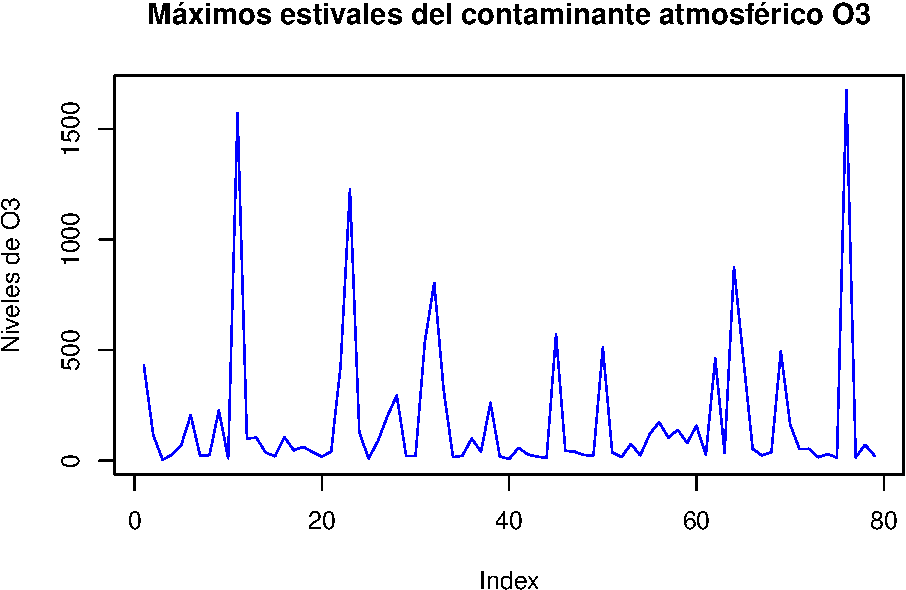
\includegraphics{Entrega_files/figure-latex/unnamed-chunk-1-1.pdf}

Como la mayoría de tests de ajustes suponen datos \(iid\), se van a
realizar dos tests de
aleatoriedad\footnote{En inglés se expresa como \textit{randomness}} a
los datos (\textit{runs up and down} y
\textit{pearman correlation of ranks}).

Se emplea la prueba de ajuste \(\chi^2\) que requiere seleccionar una
partición más o menos arbitraria de la recta real de intervalos siendo
importante que en cada intervalo haya una cantidad lo suficientemente
importante de datos de la muestra. En este sentido, se pueden tomar como
extremos de los intervalos los quintiles empíricos de la muestra. Cabe
mencionar que este test requiere estimar parámetros por el método de
Máxia Verosimilitud Categórica, que da resultado distintos al método de
Máxima Verosimilitud a secas
\footnote{Este hecho es frecuentemente ignorado y presentado erróneamente en los textos y cursos básicos de Estadística.  que da resultado distintos al método de Máxima Verosimilitud a secas. Este hecho es frecuentemente ignorado y presentado erróneamente en los textos y cursos básicos de Estadística.}.

El \(p-valor\) en runs up and down es \(0.868\) y en Spearman es
\(0.474\). Como cada dato de los 80 que disponemos es un máximo de un
centenar de observaciones, intentaremos ajustarlos a una distribución
extremal sabiendo que no necesariamente tendremos éxito. Observemos en
particular que lo que pasamos por dos tests de aleatoriedad son los 80
máximos, pero no el centenar de lecturas que forman cada uno de los 80
máximos (ni siquiera tenemos esos datos originales). Dado que
visualmente se aprecian valores muy apartados, se presume una
distribución de colas pesadas y por ese motivo se intenta un ajuste a
una Fréchet.

El test de ajuste \(\chi^2\) da un \(p-valor\) de \(0.467\) para una
Fréchet de \(\alpha=1.04\), \(\mu= -6.5\), \(\beta=44\).

Adoptando pues este modelo, un sencillo cálculo muestra que la
probabilidad de que el máximo exceda 50 es 0.455, lo cual es
absolutamente consistente con lo observado en la muestra, donde la
proporción empírica de excedencia del nivel 50 es 0.5125 con un
intervalo de confianza al \(95\%\) para esta proporción de
\((0.403, 0.622)\).

Se llega a la conclusión que hay una incidencia muy seria de niveles
moderados de riesgo (se prevee que cerca de la mitad de los puntos estén
afectados) Veremos ahora los detalles que hemos ido postergando.

Cabe mencionar que para este estudio la distribución de la variable a
incorporar en este estudio no tiene que ser degenerada, es decir
\(H(t)=0\) ó \(H(t)=1\).

\textbf{Observación 10.} Una distribución \(H\) se dice degenerada si
\(H(t)=0\) ó \(1\) para todo valor de \(t\). Representan a variables que
no son tales, si la distribución de \(X\) es degenerada, entonces \(X\)
es una constante, y no tiene sentido hacer estadística sobre \(X\), por
lo tanto sólo tienen interés para nosotros las distribuciones
no-degeneradas.

\newpage

\hypertarget{definiciuxf3n-2-distribuciuxf3n-extremal-asintuxf3tica}{%
\subsubsection{Definición 2: Distribución extremal
asintótica}\label{definiciuxf3n-2-distribuciuxf3n-extremal-asintuxf3tica}}

Si \(X_1,...,X_n\) es \(iid\) con distribución \(F\) diremos que \(H\)
no-degenerada es la Distribución Extremal Asintótica (DEA) de
\(F\)\footnote{Lo que equivale a decir que $F$ tiene $DEA\;H$.}, si
existen dos sucesiones de números reales, \(d_n\) y \(c_n>0\), tales que
la distribución de

\begin{equation}
\frac{max(X_1,...,X_n)- d_n}{c_n}\label{eq:max}
\end{equation}

tiende a \(H\) cuando \(n\) tiende a infinito.

\hypertarget{definiciuxf3n-3-supremo-esencial-de-una-variable-aleatoria-o-distribuciuxf3n}{%
\subsubsection{Definición 3: Supremo esencial de una variable aleatoria
o
distribución}\label{definiciuxf3n-3-supremo-esencial-de-una-variable-aleatoria-o-distribuciuxf3n}}

Si \(X\) tiene distribución \(F\), se llama supremo esencial de \(X\),
denotado como \(M_X\) o, indistintamente, supremo esencial de \(F\),
denotado \(MF\) a

\begin{equation}
M_X=M_F= sup\{t / F(t)<1\}\label{eq:Mx}
\end{equation}

\textbf{Observación 11:}

\begin{itemize}
\item Si $F$ es $U(a,b)$, $M_F=b$
\item Si $F$ es $Bin(m,p)$, $M_F=m$
\item Si $F$ es Normal, Exponencial, Cauchy o Poisson, $M_F$ es infinito.
\end{itemize}

\hypertarget{teorema-4}{%
\subparagraph{Teorema 4}\label{teorema-4}}

Si \(X_1,...,X_n\) es \(iid\) con distribución \(F\) cualquiera,
entonces, para \(n\) tendiendo a infinito,

\begin{equation}
X^*_n=M_F= max(X_1,...,X_n)\;tiende\;a\;M_F\label{eq:Xast}
\end{equation}

\textbf{Observación 12:}

El resultado anterior vale incluso si \(M_F\) es infinito, pero si
\(M_F\) es finito, como \(X^*n - M_F\) tiende a cero, por analogía con
el Teorema Central del Límite para promedios, buscaríamos una sucesión
\(c_n>0\) y que tienda a cero de modo tal que \((X^*n- M_F )/ c_n\)
tienda a una distribución no-degenerada y de allí surge buscar la DEA.

\hypertarget{teorema-5}{%
\subparagraph{Teorema 5}\label{teorema-5}}

Si \(F\) es una distribución con \(M_F\) finito, y para \(X\) con
distribución \(F\) se cumple que

\[
P(X=M_F)>0 
\]

entonces \(F\) NO admite DEA.

\textbf{Observación 12:}

Si \(F\) es \(Bin(m,p)\), \(M_F=m\). Si \(X\) tiene distribución \(F\),
entonces \(P( X=M_F)= P( X=m)= p_m>0\), asi que la distribucion
\(Bin(m,p)\) NO admite DEA, no se puede aproximar la distribución del
máximo de una muestra \(iid\) de variables \(Bin(m,p)\).

El Teorema anterior es un caso particular del próximo.

\hypertarget{teorema-6}{%
\subparagraph{Teorema 6}\label{teorema-6}}

Si \(F\) es una distribución con \(M_F\) finito o infinito que admite
DEA, y \(X\) tiene distribución \(F\), entonces el límite cuando \(t\)
tiende a \(M_F\) por izquierda de

\[P(X>t)/P(X \geq t)\]

debe ser 1.

\textbf{Observación 13:}

\begin{itemize}
\item Si $F$ es una distribución de Poisson de parámetro $\lambda>0$, $M_F$ es infinito. 
\item Si $k$ es un natural, entonces:
\begin{eqnarray}
\frac{P(X>k)}{P(X\geq k)} &=& \frac{P(X \geq k+1)}{P(X\geq k)} \\ \nonumber
&=& 1-\frac{P(X=k)}{P(X \geq k)} \approx 1-\left(1- \frac{\lambda}{k}\right) 
\end{eqnarray}
que tiende a $0$ cuando $k$ tiende a infinito, por lo cual $F$ NO admite DEA, o sea que no se puede aproximar el máximo de una sucesión $iid$ de variables de Poisson.
\end{itemize}

\textbf{Observación 14:}

El Teorema 6 brinda una condición NECESARIA pero NO SUFICIENTE para DEA.
Un ejemplo de ello lo aportó Von Mises, mostrando que la distribución

\[F(x)= 1- e^{(-x-sen(x))}\] cumple con la condicion del Teorema 6 pero
no admite DEA. El tema será cerrado al estudiar los dominios de
atracción maximal, en breve. Veamos ahora ejemplos donde la DEA resulta
aplicable y que ratifican algunos hechos que anticipáramos.

\textbf{Observación 15.}

Si \(F\) es \(U(0,1)\) y consideramos \(X_1,...,X_n\) \(iid\) con
distribución \(F\), resulta que la distribución de \(n( X_n^*- 1)\)
tiende a \(\Psi_1\) por lo cual la distribución uniforme tiene DEA
Weibull.

\textbf{Observación 16.}

Si \(F\) es Exponencial de parámetro 1 y consideramos \(X_1,...,X_n\)
\(iid\) con distribución \(F\), se tiene que la distribución de
\(X_n^*- log n\) tiende a \(\Lambda\) por lo cual la distribución
exponencial tiene DEA Gumbel.

\textbf{Observación 17.}

Si F es \(N(0,1)\) y consideramos \(X_1,...,X_n\) \(iid\) con
distribución \(F\), definimos la función continua y estrictamente
decreciente (para \(u>0\))

\[
g(u)=e^{(-u^2/4\pi)/u}
\]

que \(g(u)\rightarrow \infty\) cuando \(u\rightarrow 0\), y
\(g(u)\rightarrow 0\) cuando \(u\rightarrow \infty\). Por lo cual para
todo natural \(n\) existe un único valor \(u_n\) tal que

\[
g(u_n)=1/n
\]

y resulta que
\(\frac{u_n}{\sqrt{2\pi}\left (X_n^*-\frac{u_n}{\sqrt{2\pi}}\right )}\longrightarrow \Lambda\)
por lo que la distribución normal tiene DEA Gumbel.

\textbf{Observación 18:}

Si \(F\) es \(C(0,1)\) (Cauchy standard) y consideramos \(X_1,...,X_n\)
\(i.i.d\) con distribución \(F\), se tiene que la distribución de
\(\pi X^*_n/n\) tiende a \(\Phi_1\), por lo cual la distribución Cauchy
tiene DEA Fréchet.

Los ejemplos anteriores no son sorprendentes, en el sentido que aunque
presentamos FTG en una versión simplificada, dicho teorema sugiere que
cuando \(F\) admite DEA, la distribución \(H\) deberá ser una
distribución extremal. De hecho FTG resulta de combinar dos teoremas,
basadas en una nueva definición, la de distribución max-estable.

\hypertarget{definiciuxf3n-3-distribuciuxf3n-max-estables}{%
\subsubsection{Definición 3: Distribución
max-estables}\label{definiciuxf3n-3-distribuciuxf3n-max-estables}}

Si dada una \(F\) distribución, \(X\) con distribución \(F\), \(k\)
natural arbitrario y \(X_1,...,X_k\) es \(iid\) con distribución \(F\),
existen reales \(a_k\), \(b_k\) tales que \(max(X_1,...,X_k)\) tiene la
misma distribución que \(a_k X+ b_k\), \(F\) se dice
\textit{max-estable}.

El Teorema FTG resulta de superponer los dos siguientes teoremas:

\hypertarget{teorema-7}{%
\subparagraph{Teorema 7}\label{teorema-7}}

\begin{itemize}
  \item[a)] Si $F$ admite $DEA\;H$, entonces $H$ es max-estable.
  \item[b)] Si $H$ es max-estable, es la DEA de sí misma.
\end{itemize}

\hypertarget{teorema-8}{%
\subparagraph{Teorema 8}\label{teorema-8}}

Una distribución es max-estable si y solo si es
extremal\footnote{O sea Gumbel, Weibull o Fréchet}. El Teorema 7 es
bastante intuitivo y análogo a los teoremas de Lévy sobre distribuciones
estables en aproximaciones asintóticas de las distribuciones de sumas.
Para el Teorema 8 haremos enseguida un ejercicio sencillo que nos
ayudará a hacerlo creíble. Luego precisaremos, para terminar con esta
parte, cómo son las distribuciones que tienen por DEA cada uno de los
tres tipos de distribuciones extremales. Para eso precisamos recordar
algunas definiciones, como la siguiente.

\textbf{Observación 19:}

Si \(F\) y \(G\) son dos distribuciones, tienen colas equivalentes si
\(M_F=M_G\) y cuando \(t\) tiende a \(M_F\) por izquierda,
\((1-F(t))/(1-G(t))\) tiende a un valor \(c>0\). Recordando ahora cómo
se calcula la distribución del máximo de dos variables independientes,
es muy sencillo calcular la distribución del \(max\{X,Y\}\), cuando
\(X\) e \(Y\) son independientes y cada una de ellas es una distribución
extremal.

Se tiene el siguiente resultado:

\begin{longtable}[]{@{}
  >{\raggedright\arraybackslash}p{(\columnwidth - 4\tabcolsep) * \real{0.2500}}
  >{\raggedright\arraybackslash}p{(\columnwidth - 4\tabcolsep) * \real{0.2500}}
  >{\raggedright\arraybackslash}p{(\columnwidth - 4\tabcolsep) * \real{0.5000}}@{}}
\toprule\noalign{}
\begin{minipage}[b]{\linewidth}\raggedright
\(X\)
\end{minipage} & \begin{minipage}[b]{\linewidth}\raggedright
\(Y\)
\end{minipage} & \begin{minipage}[b]{\linewidth}\raggedright
\(max(X,Y)\)
\end{minipage} \\
\midrule\noalign{}
\endhead
\bottomrule\noalign{}
\endlastfoot
\textcolor{red}{Weibull} & \textcolor{red}{Weibull} &
\textcolor{red}{Weibull} \\
\textcolor[rgb]{0.0,0.5,0.0}{Weibull} &
\textcolor[rgb]{0.0,0.5,0.0}{Gumbel} &
\textcolor[rgb]{0.0,0.5,0.0}{Cola equivalente Gumbel} \\
\textcolor{blue}{Weibull} & \textcolor{blue}{Fréchet} &
\textcolor{blue}{Fréchet} \\
\textcolor[rgb]{0.0,0.5,0.0}{Gumbel} &
\textcolor[rgb]{0.0,0.5,0.0}{Weibull} &
\textcolor[rgb]{0.0,0.5,0.0}{Cola equivalente Gumbel} \\
\textcolor{red}{Gumbel} & \textcolor{red}{Gumbel} &
\textcolor{red}{Gumbel} \\
\textcolor{blue}{Gumbel} & \textcolor{blue}{Fréchet} &
\textcolor{blue}{Cola equivalente Fréchet} \\
\textcolor{blue}{Fréchet} & \textcolor{blue}{Weibull} &
\textcolor{blue}{Fréchet} \\
\textcolor{blue}{Fréchet} & \textcolor{blue}{Gumbel} &
\textcolor{blue}{Cola equivalente Fréchet} \\
\textcolor{red}{Fréchet} & \textcolor{red}{Fréchet} &
\textcolor{red}{Fréchet} \\
\end{longtable}

\textcolor{red}{\rule{1em}{1em} Las extremales son max-estables: tomar máximos de dos del mismo tipo queda en el mismo tipo.}

\textcolor[rgb]{0.0,0.5,0.0}{\rule{1em}{1em} Gumbel es más pesada que Weibull. En la cola, que es lo que cuenta para máximos, prima Gumbel.}

\textcolor{blue}{\rule{1em}{1em} Fréchet es más pesada que Gumbel y mucho más pesada que Weibull.}
\vspace{1cm}

Además, de la tabla se deduce que

\hypertarget{teorema-9}{%
\subparagraph{Teorema 9}\label{teorema-9}}

Si \(X_1,...,X_n\) independientes y cada \(X_i\) tiene uno de los tres
tipos de distribución extremal, entonces la distribución del
\(max(X_1,...,X_n)\) es:

\begin{itemize}
\item[a)] Cola equivalente a Fréchet, si alguna de las variables es Fréchet y alguna otra es Gumbel.
\item[b)]  Fréchet, si alguna es Fréchet y ninguna es Gumbel.
\item[c)]  Cola equivalente Gumbel ninguna es Fréchet pero algunas son Gumbel y otras Weibull.
\item[d)] Gumbel si todas son Gumbel.
\item[e)]  Weibull si todas son Weibull.
\end{itemize}

Vamos ahora a ver el concepto de Dominio de Atracción Maximal.

\textbf{Observación 19:}

Si \(F\) es una distribución, se dice que tiene
\textit{cola de variación regular de orden} \(-\alpha\), para
\(\alpha \geq 0\), si para todo \(t>0\), \((1-F(tx))/(1-F(x))\) tiende a
\(t^{-\alpha}\) si \(x \rightarrow \infty\). Para abreviar se dirá que
\(F\) es \(R_{-\alpha}\). Por ejemplo, para \(\alpha=3\), un caso de una
tal \(F\) es \(F(u)=1- 1/u^3\).

Por otra parte se dice que \(L\) es una
\textit{función de variación lenta} si, para todo \(t>0\),
\(L(tx)/L(x)\) tiende a 1 cuando \(x \rightarrow \infty\). Por ejemplo,
\(L(u)=log(u)\).

\newpage

\hypertarget{definiciuxf3n-4-dominio-de-atracciuxf3n-maximal}{%
\subsubsection{Definición 4: Dominio de atracción
maximal}\label{definiciuxf3n-4-dominio-de-atracciuxf3n-maximal}}

Si \(H\) es una distribución extremal (Gumbel, Weibull o Fréchet) su
Dominio de Atracción Maximal (\(DAM(H)\)) está constituído por todas las
distribuciones \(F\) que tienen \(DEA\;H\).

\hypertarget{teorema-9-dam-de-la-fruxe9chet}{%
\subparagraph{Teorema 9: DAM de la
Fréchet}\label{teorema-9-dam-de-la-fruxe9chet}}

\(F\) pertenece a la DAM de \(\Phi_{\alpha}\) si y sólo si
\(1-F(x)=x-\alpha L(x)\) para alguna \(L\) de variación lenta, lo cual
es equivalente a decir que \(F\) es \(R_{-\alpha}\).

(Un ejemplo típico seria \(1-F(x)=x^{-\alpha}\)). Además puede tomarse
\(d_n=0\) y \(c_n= n^{1/\alpha}\).

\textbf{Ejercicio 2:}

Recompruebe en función de lo anterior que la distribución de Cauchy
tiene DEA Fréchet.

\hypertarget{corolario-1-dam-de-la-fruxe9chet}{%
\subparagraph{Corolario 1: DAM de la
Fréchet}\label{corolario-1-dam-de-la-fruxe9chet}}

Si \(F\) es una distribución con densidad \(f\) que cumple que
\(xf(x)/(1-F(x))\) tiende a \(\alpha\) cuando \(x \rightarrow \infty\)
se dice que \(F\) cumple la Condición de Von Mises I. En tal caso, \(F\)
pertenece a la DAM de \(\Phi_{\alpha}\) y mas aún, la DAM de
\(\Phi_{\alpha}\) son todas las distribuciones que tienen cola
equivalente a alguna distribución que cumpla la Condición de Von Mises
I. Del DAM Fréchet y Teorema 1, surge lo siguiente.

\hypertarget{teorema-10-dam-de-la-weibull}{%
\subparagraph{Teorema 10: DAM de la
Weibull}\label{teorema-10-dam-de-la-weibull}}

\begin{itemize}
\item [a)] $F$ pertenece a la DAM de $\Psi_{\alpha}$ si y solo si $M_F$ es finito y además $$1-F(M_F -1/x)=x^{-\alpha} L(x)$$ para alguna
$L$ de variación lenta, es decir que pertenece a $R_{-\alpha}$. Observar que con el cambio de variable $u=M_F -1/x$,
resulta que $1-F(u)=(^{-}MF -u)^{\alpha} L(1/(M_F -u))$ para alguna $L$ de variación lenta, para $u< M_F$. Además puede tomarse $d_n= M_F$ y $c_n= n-\alpha$.
\item [b)] Si $F$ distribución con densidad $f$ positiva en $(a,M_F)$ para algun $a< M_F$ y $(M_F -x)f(x)/(1-F(x))$ tiende a $\alpha$ cuando $x\rightarrow M_F$, se dice que $F$ cumple la Condición de Von Mises II. En tal caso $F$ pertenece a la DAM de $\Psi_{\alpha}$ y mas aún, la DAM de $\Psi_{\alpha}$ son todas las distribuciones que tienen cola equivalente a alguna distribución que cumpla la Condición de Von Mises II.
\end{itemize}

\textbf{Ejercicio 3:}

\begin{itemize}
\item[a)] Recompruebe en función de lo anterior que la distribución uniforme tiene DEA Weibull. 
\item[b)] Encuentre la fórmula explícita de alguna distribución que no sea la uniforme y tenga DEA Weibull.
Solo resta encontra la DAM Gumbel, y eso lo aporta el próximo resultado.
\end{itemize}

\hypertarget{teorema-11-dam-de-la-gumbel}{%
\subparagraph{Teorema 11: DAM de la
Gumbel}\label{teorema-11-dam-de-la-gumbel}}

Una distribución \(F\) se dice una Función de Von Mises con función
auxiliar \(h\) si existe \(a < M_F\) (\(M_F\) puede ser finito o
infinito) tal que para algún \(c>0\) se tiene

\begin{equation}
1-F(x)= c\;exp^{{- \int_a^X \frac{1}{h(t)} dt}},
\end{equation}

con \(h\) positiva, con densidad \(h^\prime\) y \(h^\prime(x)\)
tendiendo a \(0\) para \(x\rightarrow M_F\) Se tiene entonces que la
\(DAM\) de \(\Lambda\) son todas las distribuciones que tienen cola
equivalente a alguna distribución que sea una Función de Von Mises.
Básicamente, se trata de colas más livianas que cualquier expresión del
tipo \(1/x^k\), más aún, con decaimiento \textit{del tipo exponencial},
en el sentido preciso siguiente: si como en el Teorema 11

\(1-F(x)= c\;exp^{{- \int_a^X \frac{1}{h(t)} dt}}\), entonces se tiene
\(1-F(x)= c\;exp^{-(x-a)/h(x)}\), donde la función auxiliar \(h\) es
no-decreciente y con asíntota horizontal.

Además, \(d_n\) y \(c_n\) suelen involucrar expresiones logarítmicas.
Más concretamente, \(dn = F^{-1}(1-1/n)\), \(c_n = h(d_n)\), donde
\(F^{-1}\) es la inversa generalizada (o función cuantil), definida por
\(F^{-1}(p)= inf\{t / F(t)\geq p\}\), para \(0<p<1\).

\textbf{Ejercicio 4:}

Recompruebe en función de lo anterior que la distribución exponencial y
la distribución normal tienen DEA Gumbel.

\textbf{Ejercicio 5:}

\begin{itemize}
\item[a)] Determinar si la distribución log- normal (log X es normal) tiene DEA y si la tiene, determinar cuál es su DEA. 
\item[b)] Con la ayuda de R simular una muestra de 100 datos iid, cada uno de los cuales es el máximo de 500 log-normales standard iid. Intente ajustar la distribución de la muestra de 100 datos de acuerdo a lo obtenido en la parte a).
\end{itemize}

\textbf{Ejercicio 6 ( variable acotada en DAM Gumbel) }

Tomemos tres constantes estrictamente positivas \(\alpha\), \(K\) y
\(M\) y definamos

\(F(x)= 1 – K e^{-α/(M-x)}\:\text{ para }x<M.\)

Mostrar que \(F\) es una distribución y que \(M_F= M\).

Probar que \(F\) es una función de Von Mises con función auxiliar
\(h(t)= (M-t)^2/ \alpha\) y que por lo tanto está en el DAM Gumbel.
Finalmente, si \(X_1,...,X_k\) \(iid\) con distribución \(F\), calcular
las sucesiones de reales, \(d_n\) y \(c_n>0\), tales que la distribución
de
\[(max(X_1,...,X_n)- d_n)/c_n \longrightarrow \Lambda\quad cuando \quad n\longrightarrow \infty\].

\hypertarget{corolario-2}{%
\subsubsection{Corolario 2 :}\label{corolario-2}}

Si \(F\) pertenece al \(DAM\) Gumbel, \(M_F\) es infinito, y se
considera \(X\) con distribucion \(F\), entonces \(E(X^{+k})\) es finito
para todo \(k\) natural. Los resultados antes vistos nos permiten
reconocer que distribuciones tienen \(DEA\) y si la tienen, cual es.
Cierran el tema. Adicionalmente, permiten ver con mucha precision que el
quid de esta teoría es el comportamiento de las colas de las
distribuciones, que Fréchet corresponde a las colas más pesadas, luego
la Gumbel y finalmente Weibull. Para terminar el capítulo presentaremos
la distribución de valores extremos
generalizada\footnote{GEV, por sus siglas en inglés.}, que es una forma
de compactar en una unica fórmula las tres distribuciones extremales,
debida a Jenkinson-Von Mises.

\hypertarget{definiciuxf3n-5-gev}{%
\subsubsection{Definición 5: GEV}\label{definiciuxf3n-5-gev}}

Se define a la distribución de valores extremos generalizada
\((GEV)\)\footnote{Por sus siglas en inglés relativas a Generalized Extreme Values.}
de posición \(\mu\), escala \(\beta\) e índice \(\xi\) con

\[
G(\mu,\beta,\xi) =
\begin{cases}
    e^{-(1+ \xi(t-\mu)/ \beta)(-1/ \xi)} & \text{si  } \xi \neq 0, \forall\;t\;\text{donde } 1+ \xi(t-\mu)/ \beta) >0 \\
    e^{-e^{(-(t-\mu)/ \beta)}} & \text{si  } \xi =0,\; \forall \;t \\
\end{cases}
\] \vspace{0.5cm}

En los casos en que \(\xi\) tome los siguientes valores, se tiene

\begin{align*}
 \xi=0,  & \text{ corresponde a Gumbel,} \\
 \xi< 0, &\text{ corresponde a Weibull y } \alpha=-1/ \xi \\
 \xi>0, &\text{ corresponde Fréchet y }  \alpha=1/ \xi
\end{align*}

En \(R\) existen rutinas para estimar \(\xi\) con intervalos de
confianza( por máxima verosimilitud, etc.) lo cual da formas de testear
si una extremal es Gumbel, Weibull o Fréchet.

\textbf{Observación 21:}

En algunas situaciones datos extremales pueden ajustarse a más de un
modelo. Por ejemplo, puede ocurrir que tanto ajusten los datos una
Gumbel como una Weibull. Frente a estas situaciones, no hay una receta
única de cómo proceder sino que quien está modelando debe tener claro si
corresponde volcarse hacia cálculos más pesimistas (que dan mayor
probabilidad a eventos extremos muy severos) o más optimistas.

Usualmente la opción pesimista implica privilegiar la seguridad y la
optimista la economía de recursos, pero insistimos en que la reflexión
ante cada caso es indispensable. Un poquito más adelante veremos, al
comparar un modelo Gumbel con un modelo Fréchet, que las diferencias
pueden ser sumamente drásticas.

\textbf{Observación22:}

Antes de seguir adelante, demos la respuesta a la parte \(a)\) del
Ejercicio 5. Es un ejercicio de Cálculo Diferencial sencillo mostrar que
la cola de un \(N(0,1)\), es decir \(Q(t)=P(X>t)\), donde \(X\) tiene
distribución \(N(0,1)\), es equivalente, para \(t\) tendiendo a
infinito, a la función \(\phi(t)/t\), donde \(\phi\) representa la
densidad normal típica (campana de Gauss). Basándose en esto, si se
considera ahora una variable log-normal \(Y\), tal que \(log(Y)\) es una
\(N(0,1)\), puede probarse que su cola \(R(t)=P(Y>t)\), es equivalente,
para \(t\) tendiendo a infinito, a la función \(\phi(log(t))/log(t)\).
Con un poco más de Cálculo, esta última función puede escribirse para
\(a>e\) (por ejemplo \(a=3\)), como

\begin{equation}
c\times e^{-\int_{a}^{t}1/h(s)\; ds} \quad \text{para }\: t>a
\end{equation}

donde \(c\) se expresa en función de \(a\) y
\(h(s)=\frac{s\; log(s)}{(log(s))^2+1}\) la cual cumple las hipótesis
del Teorema 11.

Se concluye entonces que la log-normal está en el \(DAM\) Gumbel, o lo
que es lo mismo, que la log- normal admite \(DEA\) Gumbel.

\textbf{Observación 23:} Tiempos y Valores de Retorno

En Ingeniería y Ciencias Ambientales, suele pensarse los eventos
extremos (por ejemplo: observación por encima de cierto valor muy alto),
en términos de tiempos de retorno (tiempo que se espere para que ocurra
un evento). Bajo las hipótesis de datos \(iid\), el tiempo de retorno
\(T\) tiene una distribución \(Geo(p)\), con \(p = P(evento)\), por lo
cual el tiempo de retorno medio es \(E(T)=1/p\) y pueden hacerse
intervalos de confianza para \(E(T)\), en la medida que exista
información de \(P(evento)\), lo cual puede obtenerse a partir de este
capítulo o de los siguientes. Cabe observar que muchas veces se utiliza
la expresión Tiempo de Retorno (TR) para \(E(T)\).

Más precisamente, \(TR(u)\), el Tiempo de retorno del valor \(u\), es el
valor esperado (o la media) del tiempo que se debe esperar para que la
variable en estudio supere el valor \(u\), es decir que
\(TR(u) = 1/P(X>u)\), si \(X\) es la variable en estudio.

Por otro la lado, en una mirada inversa, el Valor de Retorno a tiempo
\(t\), \(VR(t)\) es el valor de \(u\) para el cual \(TR(u)=t\), es decir
que \(TR(VR(t))=t\) (y también \(VR(TR(u))=u\), es decir que \(TR\) y
\(VR\) son, como funciones, inversas una de la otra).

Para \textit{bajar un poco a tierra} estos conceptos, vamos a
calcularlos y compararlos cuando la variable \(X\) es Gumbel y cuando
(con los mismos valores de posición \(\mu\) y escala \(\beta>0\)).

Comencemos por la Gumbel, recordemos que \(X\) tiene distribución
\(\Lambda( \mu,\beta)\) si \(X= \mu+\beta Y\) , donde \(Y\) tiene
distribución \(\Lambda\).

Dado entonces un valor \(\mu>0\) , otro valor \(t>0^*\) resulta que

\begin{itemize}
\item $P(X>u)=1-e^{-e{(u-\mu)/ β }}$
\item $TR(u)=1/P(X>u)$
\item $VR(t)= \mu-\beta\: log\{log\{t/(t-1)\}\}$
\end{itemize}

(ECUACIONES
G)\footnote{Cabe observar que si se supone que las observaciones son diarias (o enteras en la unidad que corresponda), los tiempos de retorno TR se redondean a enteros y los valores de $t$ en la última ecuación se toman enteros.}

Sigamos ahora por la Fréchet, recordemos que \(X\) tiene distribución
\(\Phi_{\alpha}^{( \mu,\beta)}\) si \(X= \mu+\beta Y\), donde \(Y\)
tiene distribución \(\Phi_{\alpha}\).

Dado entonces un valor \(u>0\), otro valor \(t\) entero, resulta que

\begin{itemize}
\item $P(X>u)=1-e^{ -\left \{( u- \mu)/\beta\right \}^{-\alpha}}$,
\item $TR(u)=\frac{1}{P(X>u)}$,
\item $VR(t)= \mu+ \beta\left \{log\left \{ \frac{t}{(t-1)}\right \}\right \}-\frac{1}{\alpha}$
\end{itemize}

(ECUACIONES F)

Para visualizar claramente estos resultados, tabularemos y graficaremos
los mismos usando en ambos casos:

\begin{itemize}
\item $\mu=15$
\item $\beta=10$
\item $\alpha=2.5$
\item $\xi=0.4$ no muy distante del $\xi=0$ de la Gumbel
\end{itemize}

Tanto las tablas como la gráfica muestran que el modelo Fréchet da
probabilidades mucho mayores a valores muy elevados (es más
``pesimista'', si los valores mayores representan mayores esfuerzos o
problemas).

Tratemos de ver ahora los TR para uno y otro modelo. Es claro que,
siguiendo la lógica anterior, es más ``pesimista'' el modelo que de
tiempos de retorno menores en valores elevados.

Se observa muy claramente que el modelo Fréchet es mucho más
``pesimista''.

Veamos ahora los VR. Será en este contexto más ``pesimista'' quien dé
mayores VR.

Resulta evidente el mayor ``pesimismo''del modelo Fréchet. Finalmente,
para cerrar el punto, veamos que TR y VR son efectivamente inversas.

Por ejemplo, si tomamos el tiempo \(t=90\) días, vemos que en Gumbel su
\(VR\) es \(59,942\) muy ligeramente inferior a 60. En la tabla de TR,
vemos que para el valor 60, Gumbel da TR= 91, casi igual a t=90. Si con
este mismo \(t\) vamos al modelo Fréchet, vemos que su VR es 75,537 algo
superior a 74.

En la tabla de TR vemos que para el valor 75 Fréchet da TR= 89, casi
igual a t=90.

Es decir que, salvando las ligeras diferencias fruto de que las tablas
son discretas y hay redondeos, etc., hemos corroborado que para \(t\)
días, tenemos que TR \((VR(t))=t\). Si tomamos ahora el valor 70, vemos
que en Gumbel tiene TR=245, un poco por debajo de 270, cuyo
\(VR=70,966\). En Fréchet 70 tiene \(TR=71\), más abajo que 90, que
tiene \(VR= 75,357\) bastante cercano a 70. Haciendo la salvedad de lo
artesanal y aproximado de mirar una tabla y no calcular en continuo,
queda claro que para un valor u tenemos que \(VR(TR(u))=u\).

\newpage

\subsection{POT (Peaks Over Treshold) y variantes}

\newpage

\section{Estrategia Empírica}

\newpage

\section{Referencias bibliográficas}

\hypertarget{refs}{}
\begin{CSLReferences}{1}{0}
\leavevmode\vadjust pre{\hypertarget{ref-enders}{}}%
Enders, W. 2014. \emph{Applied Econometric Time Series}. Wiley Series en
Probability y Statistics. Wiley.

\leavevmode\vadjust pre{\hypertarget{ref-notas_curso}{}}%
Perera, Gonzalo, Angel Segura, y Carolina Crisci. 2021. \emph{Curso de
estadística de datos extremales, cap. 1 a cap. 5}.

\leavevmode\vadjust pre{\hypertarget{ref-kpss}{}}%
Shin, Yongcheol, Denis Kwiatkowski, Peter Schmidt, y Peter C. B.
Phillips. 1992. {«Testing the Null Hypothesis of Stationarity Against
the Alternative of a Unit Root: How Sure Are We That Economic Time
Series Are Nonstationary?»} \emph{Journal of Econometrics} 54 (1-3):
159-78.

\leavevmode\vadjust pre{\hypertarget{ref-evd}{}}%
Stephenson, A. G. 2002. {«evd: Extreme Value Distributions»}. \emph{R
News} 2 (2): 0. \url{https://CRAN.R-project.org/doc/Rnews/}.

\end{CSLReferences}

\end{document}
